\subsection{GPU Accelerating \textit{k}mer Counting}
While different GPU accelerated \textit{k}mer counting solutions such as Gerbil \cite{gerbil} have been developed in previous work, we opted to develop our own \textit{k}mer counting method because the \textit{k}mer counting problem solved in KAGE is slightly different than the typical \textit{k}mer counting problem described in section \ref{background:kmers_and_the_kmer_counting_problem}.
Rather than counting the frequency of every observed \textit{k}mer in the input reads, or even the frequency of every observed \textit{k}mer where the frequency is larger than some threshold, KAGE is only interested in counting the observed frequencies for a predetermined set of \textit{k}mers.
This revised problem is easier to solve in practice because the memory constraints are significantly less.
In the interest of brevity, we will refer to the typical \textit{k}mer counting problem described section \ref{background:kmers_and_the_kmer_counting_problem} as \textit{full kmer counting}, and the simpler problem where we only count the frequencies of a predetermined set of \textit{k}mers as \textit{partial kmer counting} \ref{methods:gpu_accelerating_kmer_counting:partial_kmer_counting}.

\definecolor{kmer1}{RGB}{40,40,215}
\definecolor{kmer2}{RGB}{0,150,0}
\definecolor{kmer3}{RGB}{225,30,30}
\definecolor{kmer4}{RGB}{20,150,150}

\begin{figure}[H]
\begin{center}
\scalebox{1}{
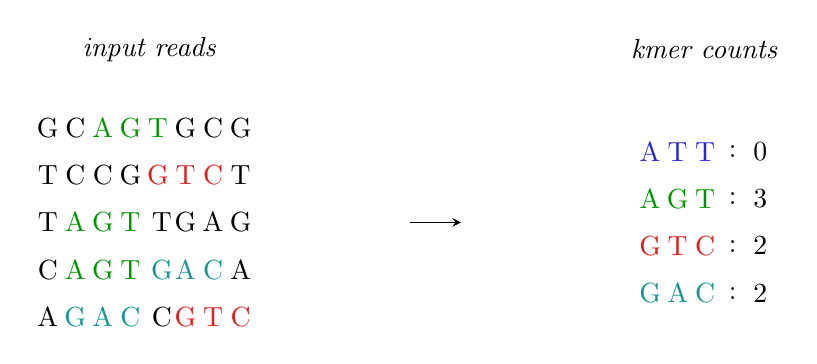
\begin{tikzpicture}
  % titles
  \node at(-0.55,3)(){\textit{input reads}};
  % read 1
  \node at(-1.85,2){G};
  \node at(-1.5,2){C};
  \node at(-1.15,2){\textcolor{kmer2}{A}};
  \node at(-.8,2){\textcolor{kmer2}{G}};
  \node at(-.45,2){\textcolor{kmer2}{T}};
  \node at(-.1,2){G};
  \node at(.25,2){C};
  \node at(.6,2){G};
  % read 2 
  \node at(-1.85,1.4){T};
  \node at(-1.5,1.4){C};
  \node at(-1.15,1.4){C};
  \node at(-.8,1.4){G};
  \node at(-.45,1.4){\textcolor{kmer3}{G}};
  \node at(-.1,1.4){\textcolor{kmer3}{T}};
  \node at(.25,1.4){\textcolor{kmer3}{C}};
  \node at(.6,1.4){T};
  % read 3 
  \node at(-1.85,.8){T};
  \node at(-1.5,.8){\textcolor{kmer2}{A}};
  \node at(-1.15,.8){\textcolor{kmer2}{G}};
  \node at(-.8,.8){\textcolor{kmer2}{T}};
  \node at(-.4,.8){T};
  \node at(-.1,.8){G};
  \node at(.25,.8){A};
  \node at(.6,.8){G};
  % read 4 
  \node at(-1.85,.2){C};
  \node at(-1.5,.2){\textcolor{kmer2}{A}};
  \node at(-1.15,.2){\textcolor{kmer2}{G}};
  \node at(-.8,.2){\textcolor{kmer2}{T}};
  \node at(-.4,.2){\textcolor{kmer4}{G}};
  \node at(-.1,.2){\textcolor{kmer4}{A}};
  \node at(.25,.2){\textcolor{kmer4}{C}};
  \node at(.6,.2){A};
  % read 5 
  \node at(-1.85,-.4){A};
  \node at(-1.5,-.4){\textcolor{kmer4}{G}};
  \node at(-1.15,-.4){\textcolor{kmer4}{A}};
  \node at(-.8,-.4){\textcolor{kmer4}{C}};
  \node at(-.4,-.4){C};
  \node at(-.1,-.4){\textcolor{kmer3}{G}};
  \node at(.25,-.4){\textcolor{kmer3}{T}};
  \node at(.6,-.4){\textcolor{kmer3}{C}};
  % Arrow
  \draw [-stealth](2.75,.8) -- (3.4,.8);
  % k-mer counts
  \node at(6.5,3)(){\textit{kmer counts}};
  % k-mer 1
  \node at(5.8,1.7){\textcolor{kmer1}{A}};
  \node at(6.15,1.7){\textcolor{kmer1}{T}};
  \node at(6.5,1.7){\textcolor{kmer1}{T}};
  \node at(6.85,1.7){:};
  \node at(7.2,1.7){0};
  % k-mer 2 
  \node at(5.8,1.1){\textcolor{kmer2}{A}};
  \node at(6.15,1.1){\textcolor{kmer2}{G}};
  \node at(6.5,1.1){\textcolor{kmer2}{T}};
  \node at(6.85,1.1){:};
  \node at(7.2,1.1){3};
  % k-mer 3 
  \node at(5.8,.5){\textcolor{kmer3}{G}};
  \node at(6.15,.5){\textcolor{kmer3}{T}};
  \node at(6.5,.5){\textcolor{kmer3}{C}};
  \node at(6.85,.5){:};
  \node at(7.2,.5){2};
  % k-mer 4 
  \node at(5.8,-.1){\textcolor{kmer4}{G}};
  \node at(6.15,-.1){\textcolor{kmer4}{A}};
  \node at(6.5,-.1){\textcolor{kmer4}{C}};
  \node at(6.85,-.1){:};
  \node at(7.2,-.1){2};
\end{tikzpicture}
}
\caption{
  In KAGE, we are only interested in counting the observed frequencies of a predefined set of \textit{k}mers, as opposed to every observed \textit{k}mer in the sequenced reads.
}
\label{methods:gpu_accelerating_kmer_counting:partial_kmer_counting}
\end{center}
\end{figure}

We here present three methods of implementing GPU accelerated \textit{k}mer counting for Python, one of which is the method used in GKAGE.

\subsubsection{Method 1: Adapting a NumPy Solution to Use CuPy} \label{methods:gpu_accelerating_kmer_counting:method1}
Our first attempt at GPU accelerating the \textit{k}mer counting process was to utilize CuPy, which was introduced in section \ref{background:cupy}.
A short reminder: CuPy is a Python package providing a GPU accelerated array library that supports most of the functionality found in NumPy \ref{background:numpy}.
In fact, CuPy can in effect be viewed as a GPU accelerated substep of NumPy, with great existing interoperability to work with both libraries in the same projects.

Another Python library, npstructures \cite{npstructures}, provides different data structures that are built on top of NumPy to provide efficient and optimized solutions.
Among others, some of the data structures provided by npstructures are a \textit{ragged} two-dimensional array object, providing an efficient two-dimensional array structure where the column lengths can vary, and a static hash table object.
The static hash table object achieves great memory efficiency by utilizing the ragged arrays to create a bucket paradigm where the size of the hash table is equal to the number of rows in the ragged array, and the bucket sizes (the columns of the ragged array) can vary.
The bucket sizes are determined by pre-computing how many of the unique keys hash to the same rows in the ragged array.
This hash table had already been utilized to count a predefined set of \textit{k}mer's frequencies, albeit on the CPU.

\textbf{(Figure illustrating how input keys hashing to the same row determines the column length (bucket size))}

To reiterate: both the ragged array and the static hash table data structures are built on top of NumPy.
As a result, their implementations are heavily reliant on NumPy's array routines that are designed to be efficient for array operations where CPU vectorization matters. 
For large array operations where data parallelism matters, the GPU is a great candidate since it can perform significantly more parallelism this way.
In addition, we know that most, if not all of the functionality used from NumPy will be supported with GPU acceleration by CuPy, through an nearly identical interface.
Thus, by replacing the NumPy functionality used with CuPy's equivalent GPU accelerated functionality, we would have a GPU accelerated hash table object in Python that could be used to count a predefined set of \textit{k}mer's frequencies.

Rather than creating a standalone package version of npstructures with GPU acceleration, we rather opted to add the possibility for GPU acceleration to the already existing package.
This meant that we needed a way to redirect NumPy function calls to their equivalent CuPy functions, preferably without having to rewrite the implementations and without making the CuPy package a dependancy for npstructures since this would in turn require users to have a GPU even to use npstructures' NumPy implementations for the CPU.
We achieved this by exploiting Python's module system.
Consider the following Python package example where our package contains two modules, both relying on NumPy for their implementations:
\begin{center}
mypackage.my\_funcs.py
\end{center}
\begin{lstlisting}[language=Python,style=pycode]
import numpy as np

def some_func_using_numpy():
  return np.zeros(10)
\end{lstlisting}

\begin{center}
mypackage.my\_classes.py
\end{center}
\begin{lstlisting}[language=Python,style=pycode]
import numpy as np

class SomeClassUsingNumPy:
  def __init__(self):
    self.data = np.zeros(10)

  def get_data(self):
    return self.data
\end{lstlisting}

Our package's initialization file imports our function and our class from their respective modules, and all functionality is usable without needing to import CuPy in either module or initialization file.
Pay attention to the \textit{set\_backend} function which takes a library as a parameter and redirects the np variable in both package modules from NumPy to this provided library.

\begin{center}
mypackage.\_\_init\_\_.py
\end{center}
\begin{lstlisting}[language=Python,style=pycode]
from .my_funcs import some_func_using_numpy
from .my_classes import SomeClassUsingNumPy 

# Swaps NumPy with lib (presumably CuPy)
def set_backend(lib):
  from . import my_funcs
  my_funcs.np = lib

  from . import my_classes
  my_classes.np = lib
\end{lstlisting}

Now in our own program, where we will import our package \textit{mypackage}, we can either directly use our package's implementation with NumPy, or we can do as the following example shows and import CuPy and set the backend in the entire package to use CuPy functionality instead of NumPy.

\begin{center}
program.py
\end{center}
\begin{lstlisting}[language=Python,style=pycode]
import cupy as cp

import mypackage
mypackage.set_backend(cp)

array = mypackage.some_func_using_numpy()
type(array) # cupy.ndarray
\end{lstlisting}

Exploiting Python's module system this way has the benefits of not making CuPy a dependancy for npstructures, and it also allows for gradual GPU support by way of only updating the backend in modules where the existing implementations are ready to be ported as is to CuPy.
By utilizing this method, we achieved GPU support for the static hash table, allowing us to use it for \textit{k}mer counting.

Drawbacks of GPU accelerating this way is that certain NumPy implementations may not be suitable for the GPU architecture, either because the implementations are in fact not entirely suited for NumPy or for array routines at all, or because the arrays are not sufficiently large to get enough benefit from the massively parallel GPU to mask the memory transfer overhead of copying data to and from the GPU.
Furthermore, some functions found in NumPy are not implemented in CuPy.
While we did not have frequent encounters with this issue, some NumPy functions that were used in npstructures were not supported in CuPy.
In these cases, this was resolved by creating custom implementations where we had the freedom to use different CuPy functionality to reproduce the wanted functionality provided by NumPy.
For classes, this can be achieved by subclassing and overriding methods where we wish to create our new custom implementations.
This method of creating custom implementations can also be deployed in cases where an implementation may be efficient and optimized in NumPy for the CPU, but inefficient for CuPy and the GPU architecture.

Consider if our package's class definition had instead been the following:
\begin{center}
mypackage.my\_classes.py
\end{center}
\begin{lstlisting}[language=Python,style=pycode]
import numpy as np

class SomeClassUsingNumPy:
  def __init__(self):
    self.data = np.zeros(10)

  def pad_with_ones(self):
    arr = self.data
    self.data = np.insert(arr, [0, len(arr)], 1)
\end{lstlisting}

In the code above, we use NumPy's insert function.
This function is, as of April 2023, not implemented in CuPy.
To circumvent this issue, we can subclass our class and create our own custom implementation, enjoying the freedom of only having to re-implementing the methods we choose.
We will create a subclass with the prefix CP:
\begin{center}
mypackage.cp\_my\_classes.py
\end{center}
\begin{lstlisting}[language=Python,style=pycode]
import numpy as np
import cupy as cp

class CPSomeClassUsingNumPy(SomeClassUsingNumPy):
  def pad_with_ones(self):
    arr = self.data
    self.data = cp.pad(arr, (1, 1), 'constant', constant_values=1)
\end{lstlisting}

In the above example, we leave the constructor as is in the parent class, and we override the \textit{pad\_with\_ones} method using a different function that is implemented in CuPy: the pad function.
Now, our two different \textit{pad\_with\_ones} implementations will behave equivalently, although our custom implementation will leverage CuPy to be GPU accelerated.

\subsubsection{Method 2: Parallel GPU Hash Table implemented in CUDA}
Our next attempt at GPU accelerating \textit{k}mer counting was to implement our own GPU accelerated hash table in native CUDA, which is Nvidia's programming platform \ref{background:graphical_processing_units:programming_model_and_cuda}.
This would grant us much granular control over our implementation compared to the method described in section \ref{methods:gpu_accelerating_kmer_counting:method1} where we constrained ourself to using CuPy's function interface.

\textbf{\large{Implementation}}

Unlike the hash table used in the previous method, this hash table uses a simpler open addressing with linear probing scheme for insertions, updates and queries.
The hash table data structure is thus a simple structure of arrays, with one array constituting the hash table keys and another the associated values (counts).
It is implemented in CUDA as a C++ class and supports the following functionalities:
\begin{compactitem}
  \item key insertion: only performed once upon initialization.
  \item key counting: for each key, if it exists in the hash table, increment the associated hash table value by one.
  \item key querying: for each key, if it exists in the hash table, fetch the associated hash table value.
\end{compactitem}

Each of these methods are implemented using custom CUDA kernels, allowing for each operation to happen for a large number of \textit{k}mers in parallel on the GPU.
Thus, the insertion, counting and query implementations all expect arrays of \textit{k}mers where a single CUDA thread is assigned to each \textit{k}mer to fulfill the insertion, count update or query.

\textbf{Hashing and Probing Scheme}

All of the kernels implemented for this hash table solution share the same linear probing scheme to resolve collisions.
Thus, when a CUDA thread is assigned a \textit{k}mer $k$ from the input array (either for insertion, count updating or querying), it will perform a murmur hash (cite murmur) to find the initial probe position $p_0$ in the hash table.

\definecolor{misscolor}{RGB}{255,215,215}
\definecolor{hitcolor}{RGB}{215,255,215}
\definecolor{countcolor}{RGB}{240,240,240}

\begin{figure}[H]
\begin{center}
\scalebox{1}{
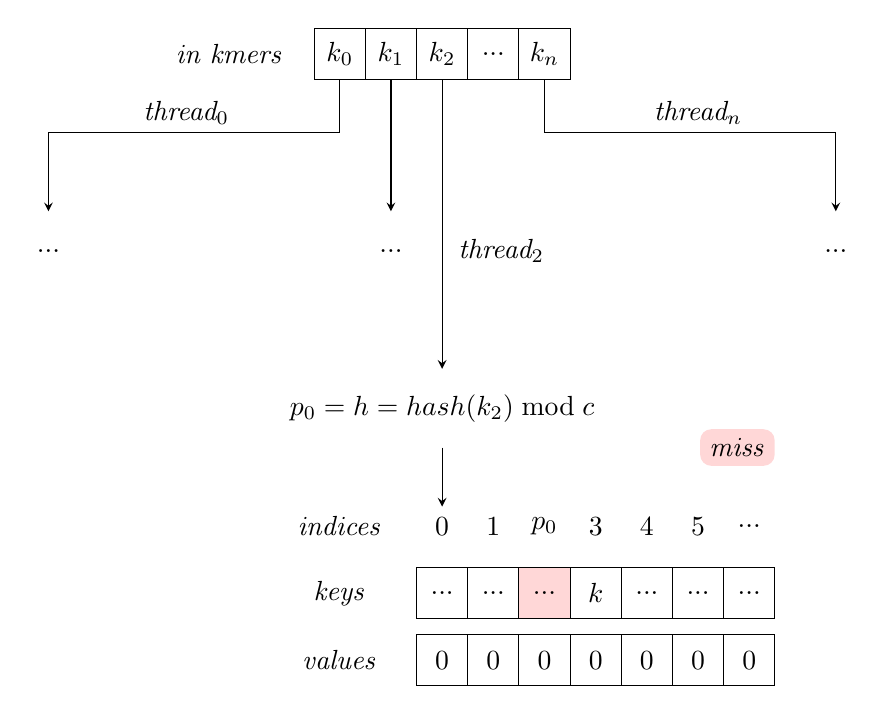
\begin{tikzpicture}
  % in kmers
  \node at(-2.7,0)(){\textit{\smaller{in kmers}}};
  \node at(-1.3,0)[draw,minimum width=0.65cm,minimum height=0.65cm](k0){\smaller{$k_0$}};
  \node at(-.65,0)[draw,minimum width=0.65cm,minimum height=0.65cm](k1){\smaller{$k_1$}};
  \node at(0,0)[draw,minimum width=0.65cm,minimum height=0.65cm](k2){\smaller{$k_2$}};
  \node at(.65,0)[draw,minimum width=0.65cm,minimum height=0.65cm](){\smaller{$...$}};
  \node at(1.3,0)[draw,minimum width=0.65cm,minimum height=0.65cm](kn){\smaller{$k_n$}};
  % CUDA threads
  % k0
  \draw [](k0) -- (-1.3,-1);
  \draw [](-1.3,-1) -- (-5,-1);
  \draw [-stealth](-5,-1) -- (-5,-2);
  \node at(-3.25,-.75)(){\textit{\smaller{thread$_0$}}};
  \node at(-5,-2.5)(){...};
  % k1
  \draw [-stealth](k1) -- (-.65,-2);
  \node at(-.65,-2.5)(){...};
  % kn
  \draw [](kn) -- (1.3,-1);
  \draw [](1.3,-1) -- (5,-1);
  \draw [-stealth](5,-1) -- (5,-2);
  \node at(3.25,-.75)(){\textit{\smaller{thread$_n$}}};
  \node at(5,-2.5)(){...};
  % k2
  \draw [-stealth](k2) -- (0,-4);
  \node at(.75,-2.5)(){\textit{\smaller{thread$_2$}}};
  % hash
  \node at(0,-4.5)(){\smaller{\textit{$p_0=h=hash(k_2) \bmod c$}}};
  \draw [-stealth](0,-5) -- (0,-5.75);

  % probe 1
  \node at(3.75,-5)[fill=misscolor,rounded corners](miss){\textit{\smaller{miss}}};
  % titles
  \node at(-1.3,-6)(){\textit{\smaller{indices}}};
  \node at(-1.3,-6.85)(){\textit{\smaller{keys}}};
  \node at(-1.3,-7.7)(){\textit{\smaller{values}}};
  % indices
  \node at(0,-6)[minimum width=0.65cm,minimum height=0.65cm](){\smaller{$0$}};
  \node at(.65,-6)[minimum width=0.65cm,minimum height=0.65cm](){\smaller{$1$}};
  \node at(1.3,-6)[minimum width=0.65cm,minimum height=0.65cm](){\smaller{$p_0$}};
  \node at(1.95,-6)[minimum width=0.65cm,minimum height=0.65cm](){\smaller{$3$}};
  \node at(2.6,-6)[minimum width=0.65cm,minimum height=0.65cm](){\smaller{$4$}};
  \node at(3.25,-6)[minimum width=0.65cm,minimum height=0.65cm](){\smaller{$5$}};
  \node at(3.9,-6)[minimum width=0.65cm,minimum height=0.65cm](){\smaller{$...$}};
  % keys
  \node at(0,-6.85)[draw,minimum width=0.65cm,minimum height=0.65cm](){\smaller{$...$}};
  \node at(.65,-6.85)[draw,minimum width=0.65cm,minimum height=0.65cm](){\smaller{$...$}};
  \node at(1.3,-6.85)[draw,minimum width=0.65cm,minimum height=0.65cm,fill=misscolor](){\smaller{$...$}};
  \node at(1.95,-6.85)[draw,minimum width=0.65cm,minimum height=0.65cm](){\smaller{$k$}};
  \node at(2.6,-6.85)[draw,minimum width=0.65cm,minimum height=0.65cm](){\smaller{$...$}};
  \node at(3.25,-6.85)[draw,minimum width=0.65cm,minimum height=0.65cm](){\smaller{$...$}};
  \node at(3.9,-6.85)[draw,minimum width=0.65cm,minimum height=0.65cm](){\smaller{$...$}};
  % values
  \node at(0,-7.7)[draw,minimum width=0.65cm,minimum height=0.65cm](){\smaller{$0$}};
  \node at(.65,-7.7)[draw,minimum width=0.65cm,minimum height=0.65cm](){\smaller{$0$}};
  \node at(1.3,-7.7)[draw,minimum width=0.65cm,minimum height=0.65cm](){\smaller{$0$}};
  \node at(1.95,-7.7)[draw,minimum width=0.65cm,minimum height=0.65cm](){\smaller{$0$}};
  \node at(2.6,-7.7)[draw,minimum width=0.65cm,minimum height=0.65cm](){\smaller{$0$}};
  \node at(3.25,-7.7)[draw,minimum width=0.65cm,minimum height=0.65cm](){\smaller{$0$}};
  \node at(3.9,-7.7)[draw,minimum width=0.65cm,minimum height=0.65cm](){\smaller{$0$}};
  
\end{tikzpicture}
}
\caption{
  ...
}
\label{methods:gpu_accelerating_kmer_counting:method2:figures:probing_scheme}
\end{center}
\end{figure}

\textbf{Insertions}

...

\subsubsection{Method 3: Parallel GPU Hash Table without CUDA or C++}
...

\subsection{GPU Accelerating \textit{k}mer Hashing}

